\newcommand{\pwidth}{.95\textwidth}
\subsection{Rectifier}
The simulated output from the half-wave rectifier circuit is shown in
Figure~\ref{fig:halfwavePlotV}.  As is shown, the maximum input voltage
is~\SI{17.401}{\volt} (zero-to-peak), implying an RMS voltage
of~\SI{12.3}{\volt} --- just one tenth of a volt higher than the designed value.
%
\begin{figure}[H]
	\centering
	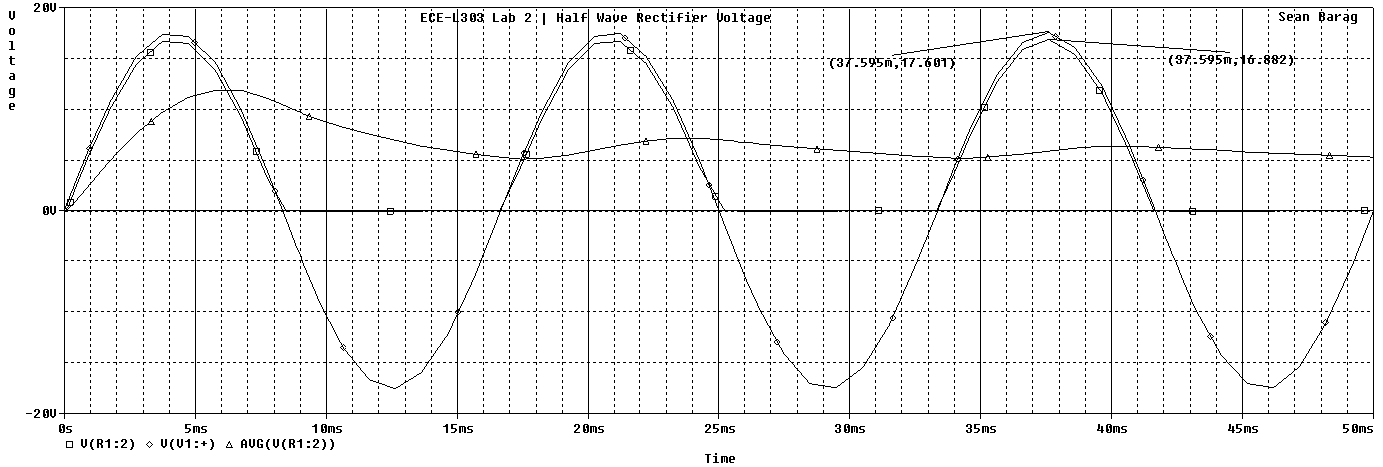
\includegraphics[width=\pwidth]{img/plot/halfwavePlot.PNG}
	\parbox{\pwidth}{
	\caption[PSpice Plot --- Half-wave Rectifier (Voltage)]{PSpice simulated
		input and output voltages as a function of time, as well as the average
		value of the output.  This data corresponds to the circuit in
		Figure~\ref{fig:schem1}.}
	\label{fig:halfwavePlotV}}
\end{figure}
%
Similarly, the output had a peak value of~\SI{16.648}{\volt} (zero-to-peak).
After dividing by~$\pi$, the average voltage was found to be~\SI{5.29}{\volt}
--- roughly~\SI{0.3}{\volt} lower than it should be.  The average value of the
output is also plotted on these axes.  As is expected, its value
approaches~\SI{5.29}{\volt} as more input cycles pass.  The decreased average
value is caused by the~\SI{0.7}{\volt} potential drop across the diode required
to turn it on, which is evident in the difference between the peak input and
output values.

An evaluation of power dissipation was also conducted, to ensure that certain
parts would be safe to use.  A plot of power dissipation over time is shown in
Figure~\ref{fig:halfwavePlotW}.
%
\begin{figure}[H]
	\centering
	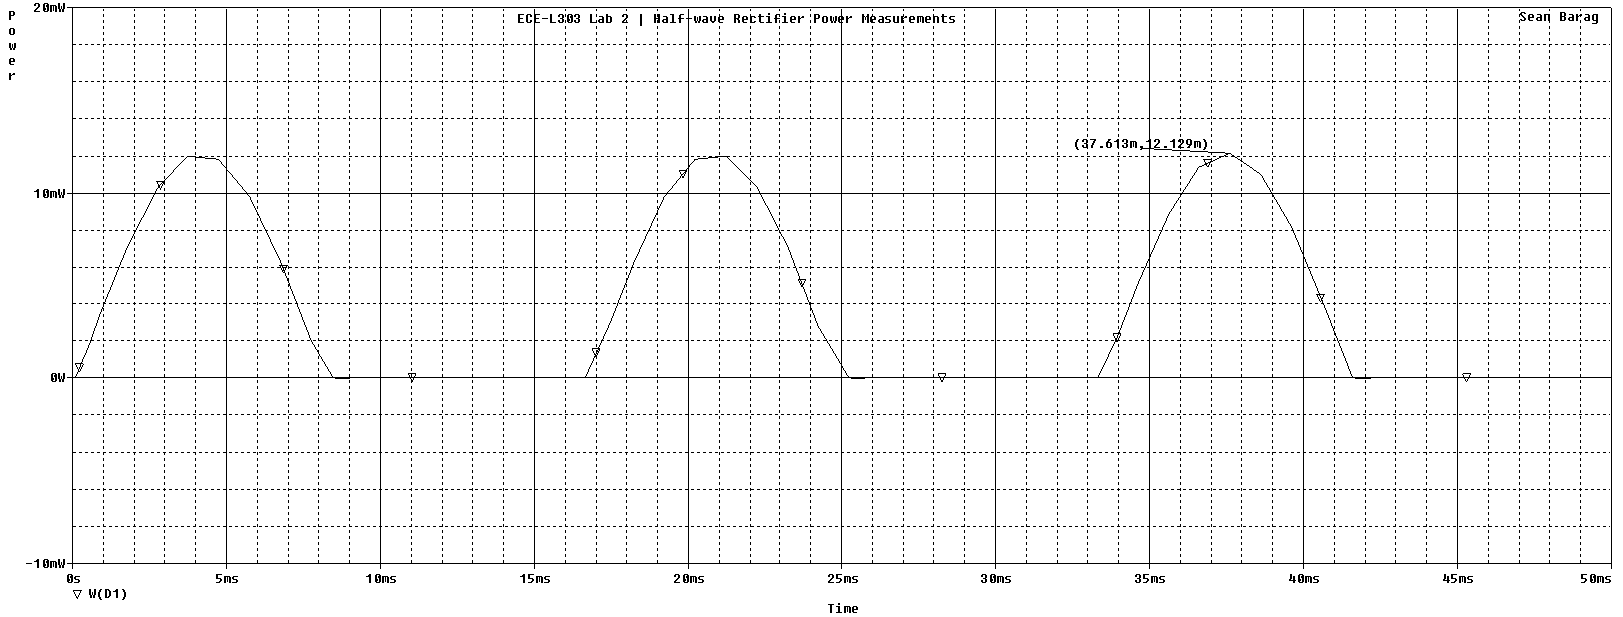
\includegraphics[width=\pwidth]{img/plot/halfwavePowerPlot.PNG}
	\parbox{\pwidth}{
	\caption[PSpice Plot --- Half-wave Rectifier (Power)]{Simulated power
		dissipation for the half-wave rectifier's diode shown in
		Figure~\ref{fig:schem1}.}
	\label{fig:halfwavePlotW}}
\end{figure}
%
The maximum power dissipated by the diode is shown as~\SI{12.129}{\milli\watt}.
Any diode with a maximum power dissipation of even one-eighth of a Watt will be
more than sufficient for this circuit.

\subsection{Voltage Regulator}
The regulated output of the zener diode-based regulator, as simulated by
PSpice, is plotted in Figure~\ref{fig:zenerPlotV}.  As is shown, the diode
begins to regulate the voltage when the input is\SI{10.085}{\volt}.
%
\begin{figure}[H]
	\centering
	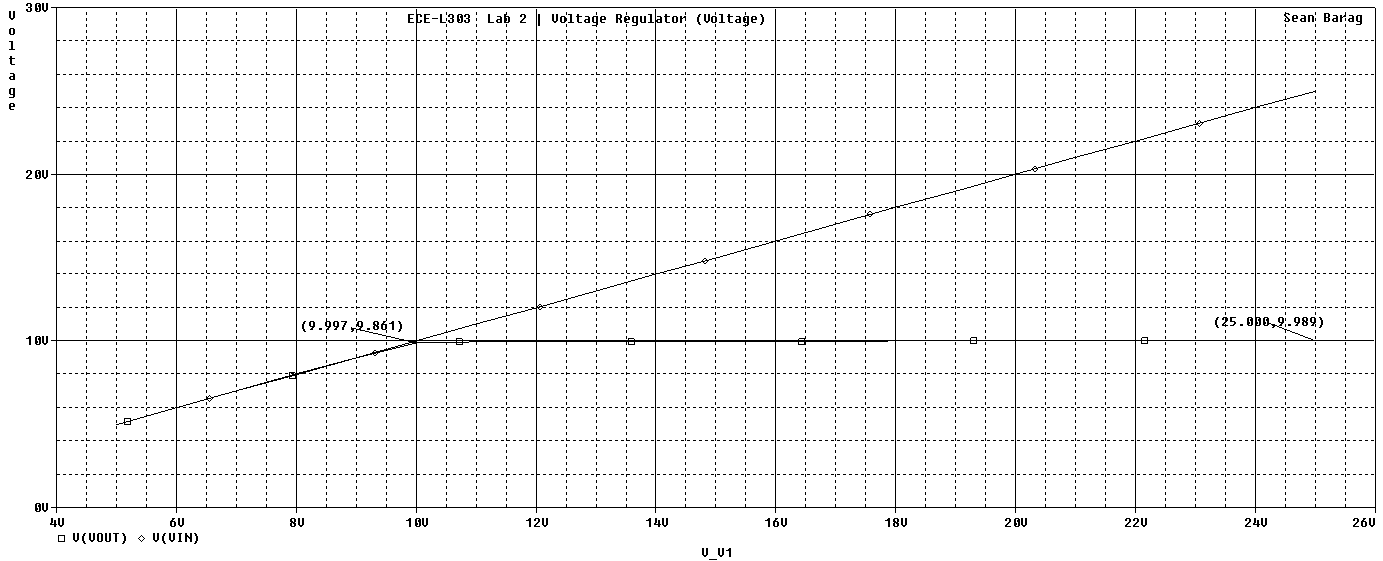
\includegraphics[width=\pwidth]{img/plot/zenerPlot.PNG}
	\parbox{\pwidth}{
	\caption[PSpice Plot --- Voltage Regulator (Voltage)]{Plot of simulated
	voltage regulator output for the circuit shown in Figure~\ref{fig:schem3}.
	The output is clearly regulated for all inputs above~$\sim$\SI{10}{\volt}.}
	\label{fig:zenerPlotV}}
\end{figure}
%
While regulated, the output voltage remains near the designed value of
~\SI{10}{\volt} DC, but tends to increase slightly due to a decrease in
efficiency in the diode as it heats up.  Where regulation begins, the output
measures~\SI{9.86}{\volt}, a value that increases to just~\SI{9.98}{\volt}
where the input voltage is~\SI{25}{\volt}.  This implies an increase of
just~\SI{8}{\milli\volt\per\volt}.

A power dissipation analysis was conducted for the zener diode circuit, as was
conducted with the half-wave rectifier.  Using PSpice's power probe, a plot of
the power dissipated by both the resistor and the zener diode was created.
This plot is reproduced below in Figure~\ref{fig:zenerPlotW}.
%
\begin{figure}[H]
	\centering
	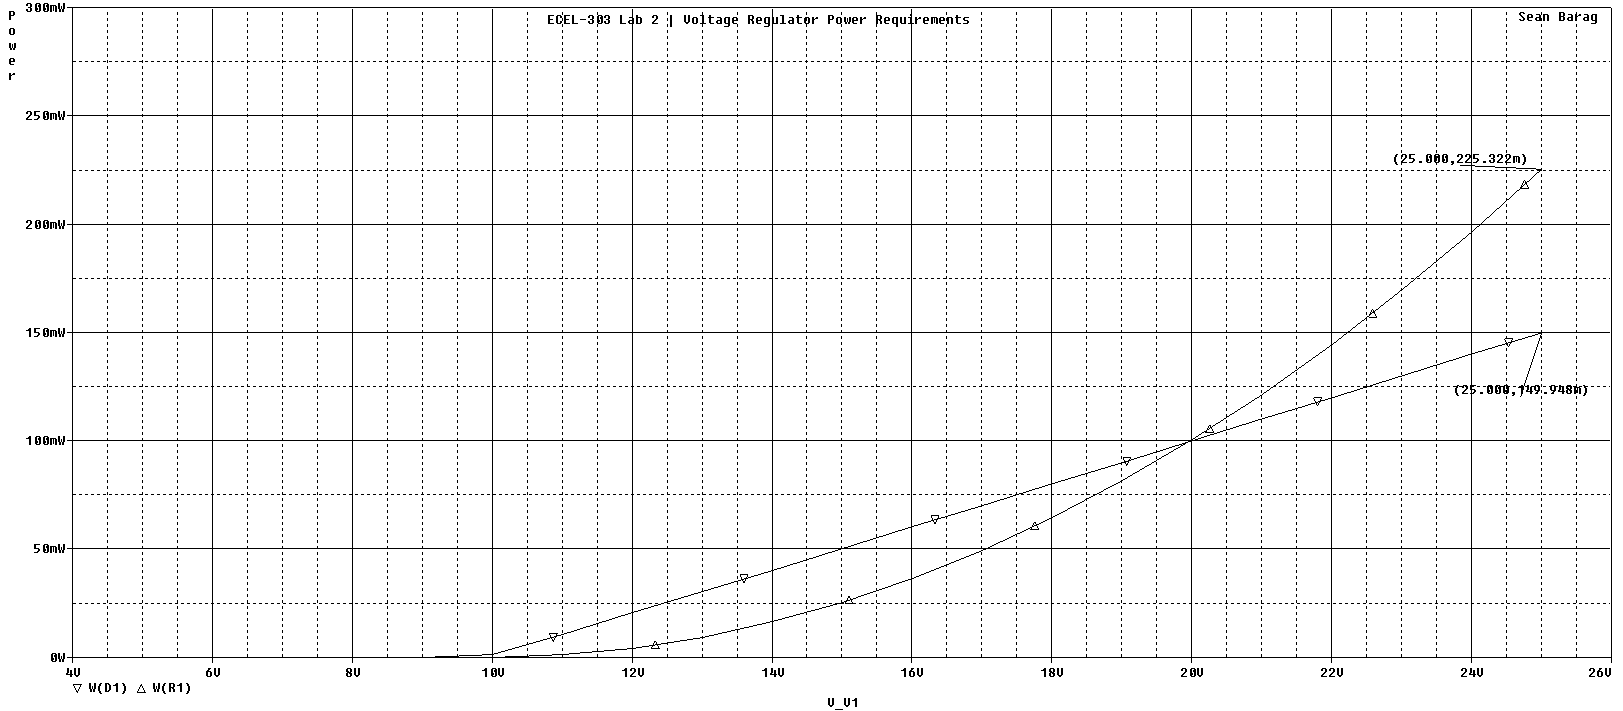
\includegraphics[width=\pwidth]{img/plot/zenerPowerPlot.PNG}
	\parbox{\pwidth}{
	\caption{}
	\label{fig:zenerPlotW}}
\end{figure}
%
According to the plot and PSpice's associated data, the maximum amount of power
dissipation required for the zener diode to be used safely
is~\SI{150}{\milli\watt}.  As such, a diode with maximum power rating of just a
quarter-watt can be safely used for this experiment.  Since the power
dissipated through the zener diode increases linearly, it can also be used for
input values up to and above~\SI{30}{\volt}.

The maximum value power dissipated through the resistor
is~\SI{225}{\milli\watt}, implying that a standard~\SI{1/4}{\watt} resistor
will be sufficiently capable for the range of inputs simulated here.  It should
be noted however that the power dissipated by the resistor follows a quadratic
increase, as is expected by the fact that power dissipated by an element is
simply the product of its resistance and the square of the current flowing
through it.  Since the resistance is constant and the current through the
device increases linearly according to Ohm's Law, it makes intuitive sense for
the power to increase quadratically.  As a result, it is not advised that a
quarter-Watt resistor be used for this experiment if the maximum input voltage
will be larger than~\SI{25}{\volt}.

\subsection{Constant Current Source}
PSpice was used to simulate two different constant current sources: one driven
by a~\SI{16}{\volt} source and one driven by a~\SI{32}{\volt} source.  The
resulting output voltage where the voltage source measures~\SI{16}{\volt} is
shown in Figure~\ref{fig:ccPlot16}.
%
\begin{figure}[H]
	\centering
	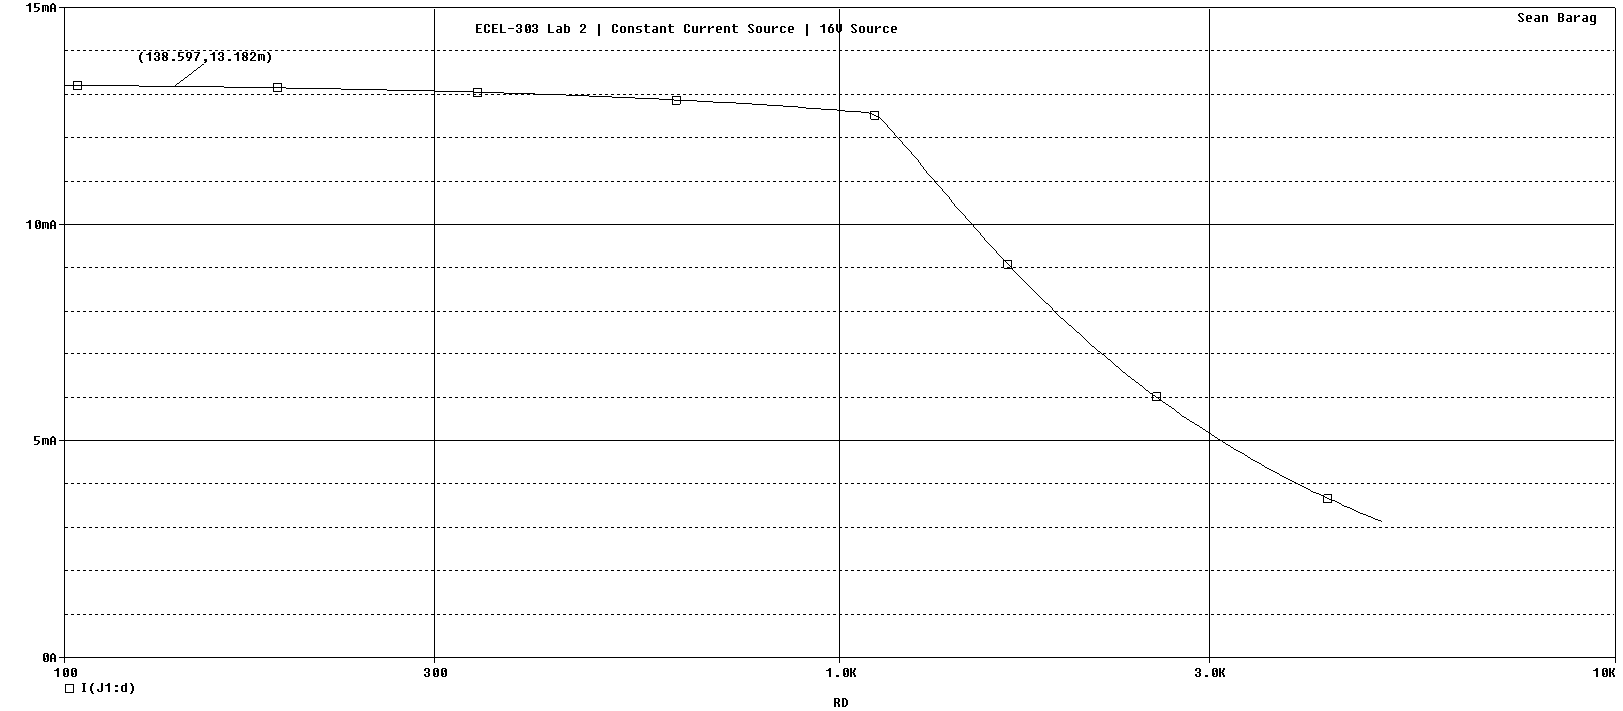
\includegraphics[width=\pwidth]{img/plot/constantCurrent16Plot.PNG}
	\parbox{\pwidth}{
	\caption{}
	\label{fig:ccPlot16}}
\end{figure}
%
By JFET used in this simulation is capable of regulating the current through
its drain util the drain resistance reaches roughly~\SI{1.15}{\kilo\ohm}.  For
loads above this value, the output current begins to decrease at a rate
of~\SI{0.002}{\milli\ampere\per\kilo\ohm}.

A similar effect occurred with the~\SI{32}{\volt} version of this circuit,
shown in Figure~\ref{fig:ccPlot32}.  Once the load resistance crosses a
threshold, the JFET begins to steadily lose its ability to regulate the current
flowing through the drain.
%
\begin{figure}[H]
	\centering
	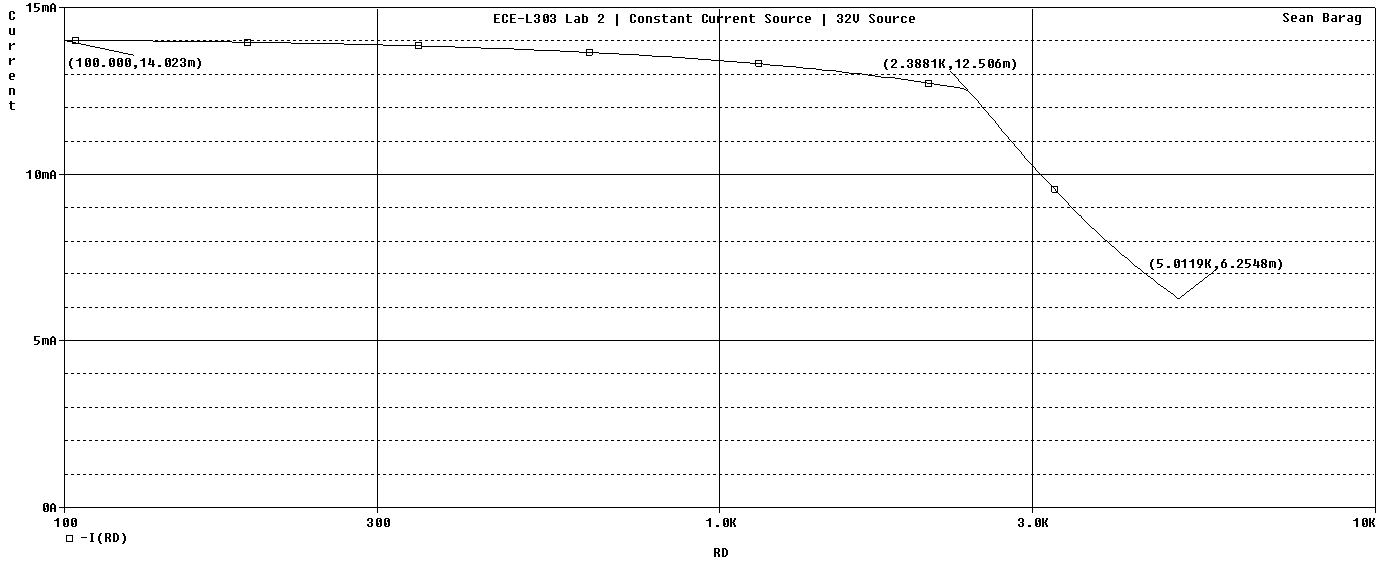
\includegraphics[width=\pwidth]{img/plot/constantCurrent32Plot.PNG}
	\parbox{\pwidth}{
	\caption{}
	\label{fig:ccPlot32}}
\end{figure}
%
Compared to the~\SI{16}{\volt} source, this simulation shows a threshold
resistance of~\SI{2.4}{\kilo\ohm}.  For all greater resistances, the current
through the drain decreases at roughly~\SI{2.4}{\milli\ampere\per\kilo\ohm}.

\subsection{High Input Resistance Buffer Amplifier}
\begin{figure}[H]
	\centering
	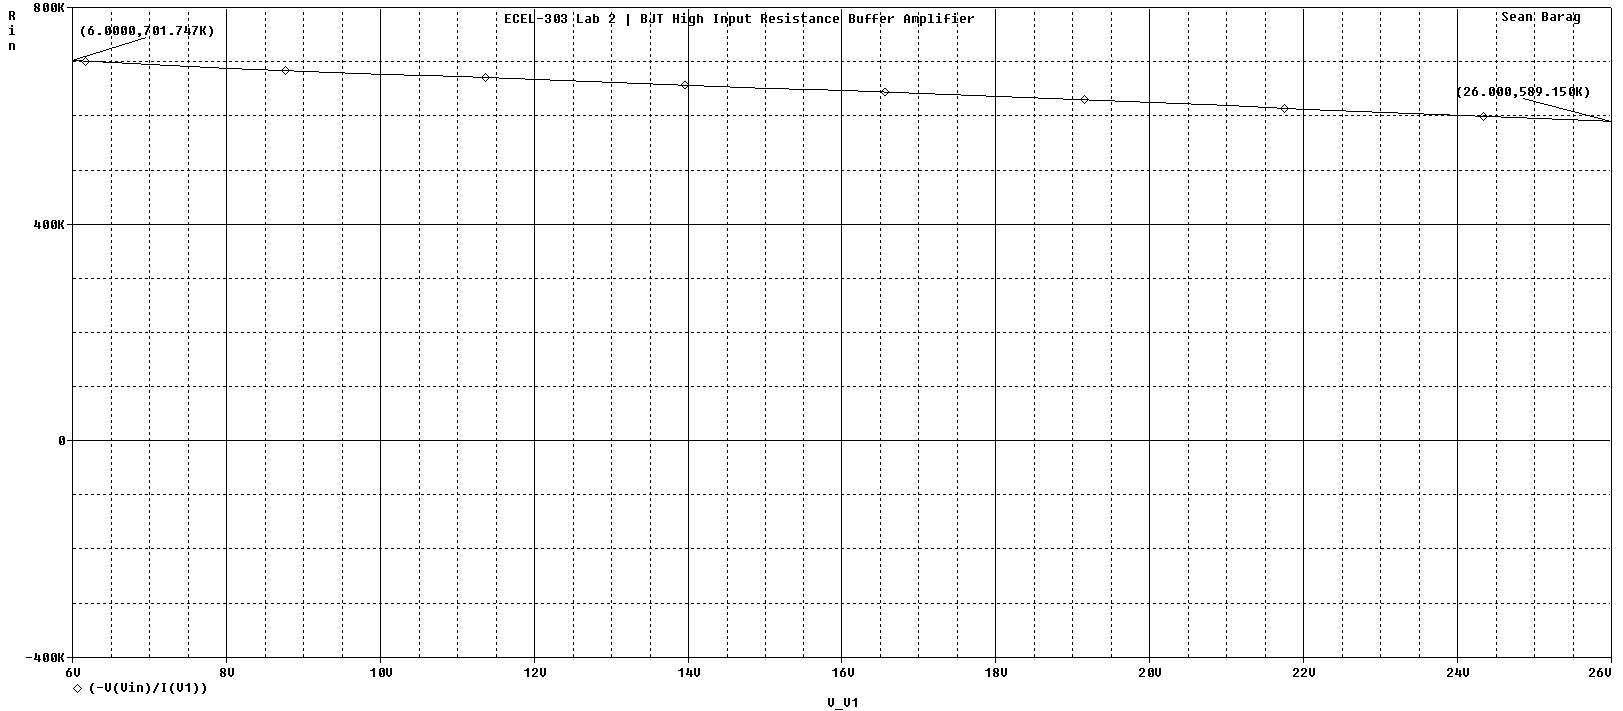
\includegraphics[width=\pwidth]{img/plot/bjtPlotR.PNG}
	\parbox{\pwidth}{
	\caption{}
	\label{fig:bjtPlotR}}
\end{figure}

\begin{figure}[H]
	\centering
	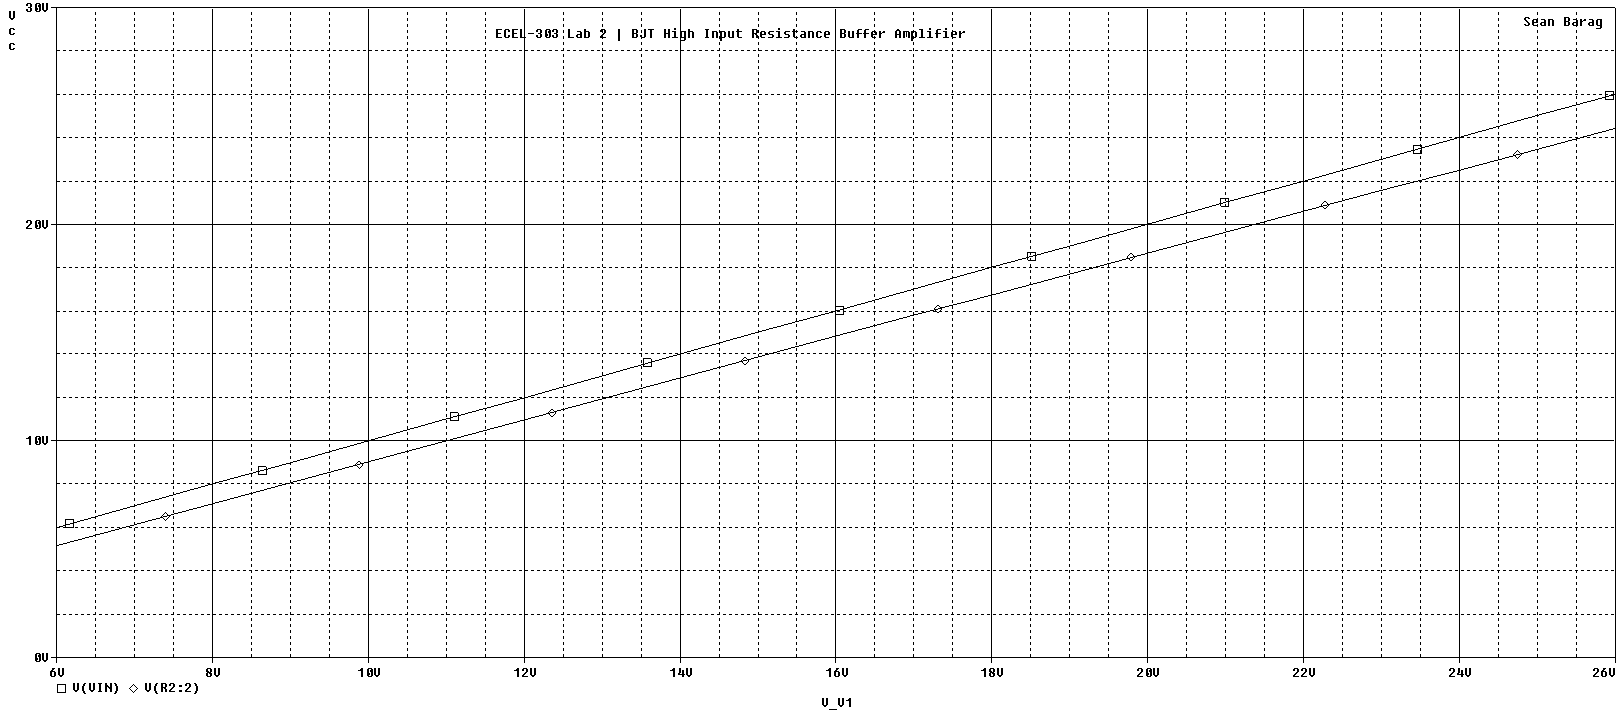
\includegraphics[width=\pwidth]{img/plot/bjtPlotV.PNG}
	\parbox{\pwidth}{
	\caption{}
	\label{fig:bjtPlotV}}
\end{figure}
